\begin{frame}[fragile]

  {\Huge Tuning}

  \vspace{10pt}

  {\large Using Kokkos' autotuning hooks.}

  \vspace{20pt}

  \textbf{Learning objectives:}
  \begin{itemize}
    \item {Why do we need tuning?}
    \item {What are Input and Output Variables?}
    \item {How to register parameters for tuning.}
    \item {Using the APEX Tuner.}
    \item {Using the Apollo Tuner.}
  \end{itemize}

  \vspace{-20pt}

\end{frame}

%==========================================================================


\begin{frame}[fragile]{Why Tuning?}
Lets look at the canonical implementation for SPMV in Kokkos:
\begin{code}[keywords={int,parallel_for,auto,parallel_reduce,TeamThreadRange,TeamPolicy,ThreadVectorRange,double}]
int rows_per_team = ...;
parallel_for("SPMV",TeamPolicy<>(nrows/rows_per_team,
  team_size,vector_length),
  KOKKOS_LAMBDA(auto const team_t& team) {
  int start_row = team.league_rank()*rows_per_team;
  parallel_for(
    TeamThreadRange(team,start_row,start_row+rows_per_team),
    [&](int row) {
      int idx_begin = a.offsets(row); 
      int idx_end = a.offsets(row+1);
      parallel_reduce(ThreadVectorRange(team,idx_begin,idx_end),
      [&](int i, double& lsum) {
        lsum += A.value(i) * x(A.idx(i));
      },y(row));
    }); 
  });
\end{code}
\end{frame}

\begin{frame}[fragile]{Why Tuning?}
There are three free parameters which determine performance:
 
\hspace{10pt} \textbf{rows\_per\_team} \hspace{10pt} \textbf{team\_size} \hspace{10pt} \textbf{vector\_length}

\vspace{5pt}
These parameters depend most on three factors:
\begin{itemize}
  \item Which architecture are you on?
  \item How many rows are in A?
  \item How many non-zeros are in A?
\end{itemize}
\end{frame}

%==========================================================================

\begin{frame}[fragile]{Why Tuning}
\textbf{Finding the right parameters is a daunting task.}

Heuristics are possible, but they have to change all the time
\begin{itemize}
  \item KokkosKernels' heuristic for NVIDIA K80 failed on V100
  \item Now AMD GPUs and Intel GPUs are coming. 
\end{itemize}

\pause
\vspace{10pt}
What if you could auto tune these parameters instead?

\vspace{5pt}
What information would you need to provide and what comes out? Need:

\pause
\vspace{5pt}
\begin{itemize}
  \item Context information, such as problem sizes.
  \item To be able to provide multiple inputs of different types.
  \item To tune multiple correlated parameters.
  \item Different tuning strategies in different areas.
\end{itemize}

\pause
\begin{block}{Kokkos Tuning}
Kokkos Tuning provides a flexible runtime auto tuning interface.
\end{block}
\end{frame}


\begin{frame}[fragile]{Tuning a Parameter}
\textbf{Kokkos' Tuning Infrastructure is very flexible.}

\pause
\vspace{5pt}
\textit{Which makes it right now more complex than is desirable.}

We will glance over some aspects here and give you the most important info for simple tuning tasks.

\pause
\vspace{10pt}
Kokkos Tuning has four fundamental concepts:
\begin{itemize}
  \item \texttt{Input-Types}: Descriptors for the type of input information for tuning tasks
  \item \texttt{Output-Types}: Descriptors of output variables for tuning tasks
  \item \texttt{Variable-Values}: Instances of \texttt{Input-Types} or \texttt{Output-Types}
  \item \texttt{Contexts:} Marker for tuning scopes. 
\end{itemize}
\end{frame}

\begin{frame}[fragile]{Types}
The types for input variables and output variables describe what makes sense to do with a variable
\begin{itemize}
  \item Not types in the C++ sense
  \item These types can contain runtime information such as candidate sets.
\end{itemize}

\pause
\vspace{5pt}
\textbf{Huh? Where is this coming from?}

Think about the different optimization spaces of variables:
\begin{itemize}
\item Discrete sets, only specific values make sense: e.g. vector length 2, 4, 8, 16
\item Continuous ranges, all values in a range $0-N$ are valid.
\item Statistical semantics, is the search space logarithmic or linear?
\end{itemize}

Often you'll have a simple case, for which we will provide helper functions.

\pause
\textbf{Tuning Variables (both input and output) need to accomodate these situations.}

\vspace{5pt}
\textit{We will discuss this later}
\end{frame}

\begin{frame}[fragile]{Tuning a single variable}
\textit{Kokkos Provided API will be highlighted, and is in the namespace \texttt{Kokkos::Tools::Experimental}}

\vspace{5pt}
\textbf{Start by creating the types (helper functions discussed later):}
\begin{code}
std::vector<int64_t> candidates = {0, 3, 7, 11};
size_t tuning_candidate_type_id = 
  create_tuning_output_type("values",candidates);
size_t tuning_input_type_id = 
  create_tuning_input_type("kernels");
\end{code}

\textbf{Next create variables for the inputs:}
\begin{code}[keywords={VariableValue,make_variable_value}]
VariableValue input_A = 
  make_variable_value(tuning_input_type_id,"A");
VariableValue input_B = 
  make_variable_value(tuning_input_type_id,"B");
\end{code}

\textbf{The actual tuning region is scoped through a context:}
\begin{code}[keywords={get_new_context_id,begin_context,end_context}]
size_t context_1 = get_new_context_id();
begin_context(context_1);
// This is the tuned region
end_context(context_1);
\end{code}
\end{frame}


\begin{frame}[fragile]{Tuning a single variable}
The context scope defines both the timing for the tuning operation and the scope in which to set input variables and obtain output (tuned) variables:

\begin{code}[keywords={get_new_context_id,begin_context,end_context,set_inpute_values,request_output_values,set_input_values}]
size_t context_1 = get_new_context_id();
begin_context(context_1);
set_input_values(context_1, 1, &input_value_A);
request_output_values(context_1, 1, &tuned_value);
end_context(context_1);
\end{code}

\pause
In this case we used a \texttt{Categorical} input value
\begin{itemize}
  \item Essentially just marks a code path as used here.
  \item But for SPMV optimal vector length depends on row lengths!
  \begin{itemize}
    \item If there is only 1 matrix: categorical works
    \item Else need numerical input value, where output mapping depends on input potentially not just as a lookup.
  \end{itemize}
\end{itemize}

\pause
We also only used one input and one output value:
\begin{itemize}
	\item Interface takes pointers to arrays for multiple \texttt{VariableValue}!
\end{itemize}
\end{frame}

%==========================================================================

\begin{frame}[fragile]{Helper Functions}

The code we demonstrated before used helper functions. We'll show their
implementation to help demonstrate some details.

\begin{code}[keywords={get_new_context_id,begin_context,end_context,VariableInfo,
	               StatisticalCategory,kokkos_value_catgorical,ValueTYpe,
		       kokkos_value_int64,kokkos_value_double,valueQuantity,CandidateValueType,
		       kokkos_value_set,make_candidate_set,declare_output_type}]
template <class T>
size_t create_tuning_output_type(
    const char* name,
    std::vector<T>& candidate_values) {
  using Kokkos::Tools::Experimental;
  VariableInfo tuningVariableInfo;
  tuningVariableInfo.category =
      StatisticalCategory::kokkos_value_categorical;
  tuningVariableInfo.type = std::is_integral<T>::value ?
      ValueType::kokkos_value_int64 :
      ValueType::kokkos_value_double;
  tuningVariableInfo.valueQuantity =
      CandidateValueType::kokkos_value_set;
  tuningVariableInfo.candidates = make_candidate_set(
      candidate_values.size(),
      candidate_values.data());  
  return declare_output_type(name, tuningVariableInfo);
}
\end{code}
\end{frame}
\begin{frame}[fragile]{Helper Functions Continued}

\begin{code}[keywords={get_new_context_id,begin_context,end_context,VariableInfo,
	               StatiscalCategory,kokkos_value_categorical,kokkos_value_string,
		       kokkos_value_unbounded,declare_inpute_type,valueQuantity}]
size_t create_tuning_input_type(const char* name) {
  using Kokkos::Tools::Experimental;
  VariableInfo info;
  info.category = StatisticalCategory::kokkos_value_categorical;
  info.type = ValueType::kokkos_value_string;
  info.valueQuantity = kokkos_value_unbounded;
  return declare_input_type(name, info);
}
\end{code}


\end{frame}

\begin{frame}[fragile]{APEX: Runtime Auto-tuning for Kokkos Applications} 
\begin{itemize}
   \item APEX: Autonomic Performance Environment for eXascale 
   \item Associated with TAU profiling library, reusing its codebase.
   \item Provides auto-tuning during Kokkos application's execution, e.g., at every invocation of a \texttt{Kokkos::parallel\_for()}
   \item Search for best-performing tuning parameter values via simulated annealing or genetic search. 
\end{itemize}

\pause
How to use APEX:\\
	\begin{code}[mathescape=false]
apex_exec --apex:kokkos-tuning ./Executable.exe ARGS
\end{code}
\end{frame}

\begin{frame}[fragile]{APEX Speeds Up Kokkos Applications}

\begin{figure}
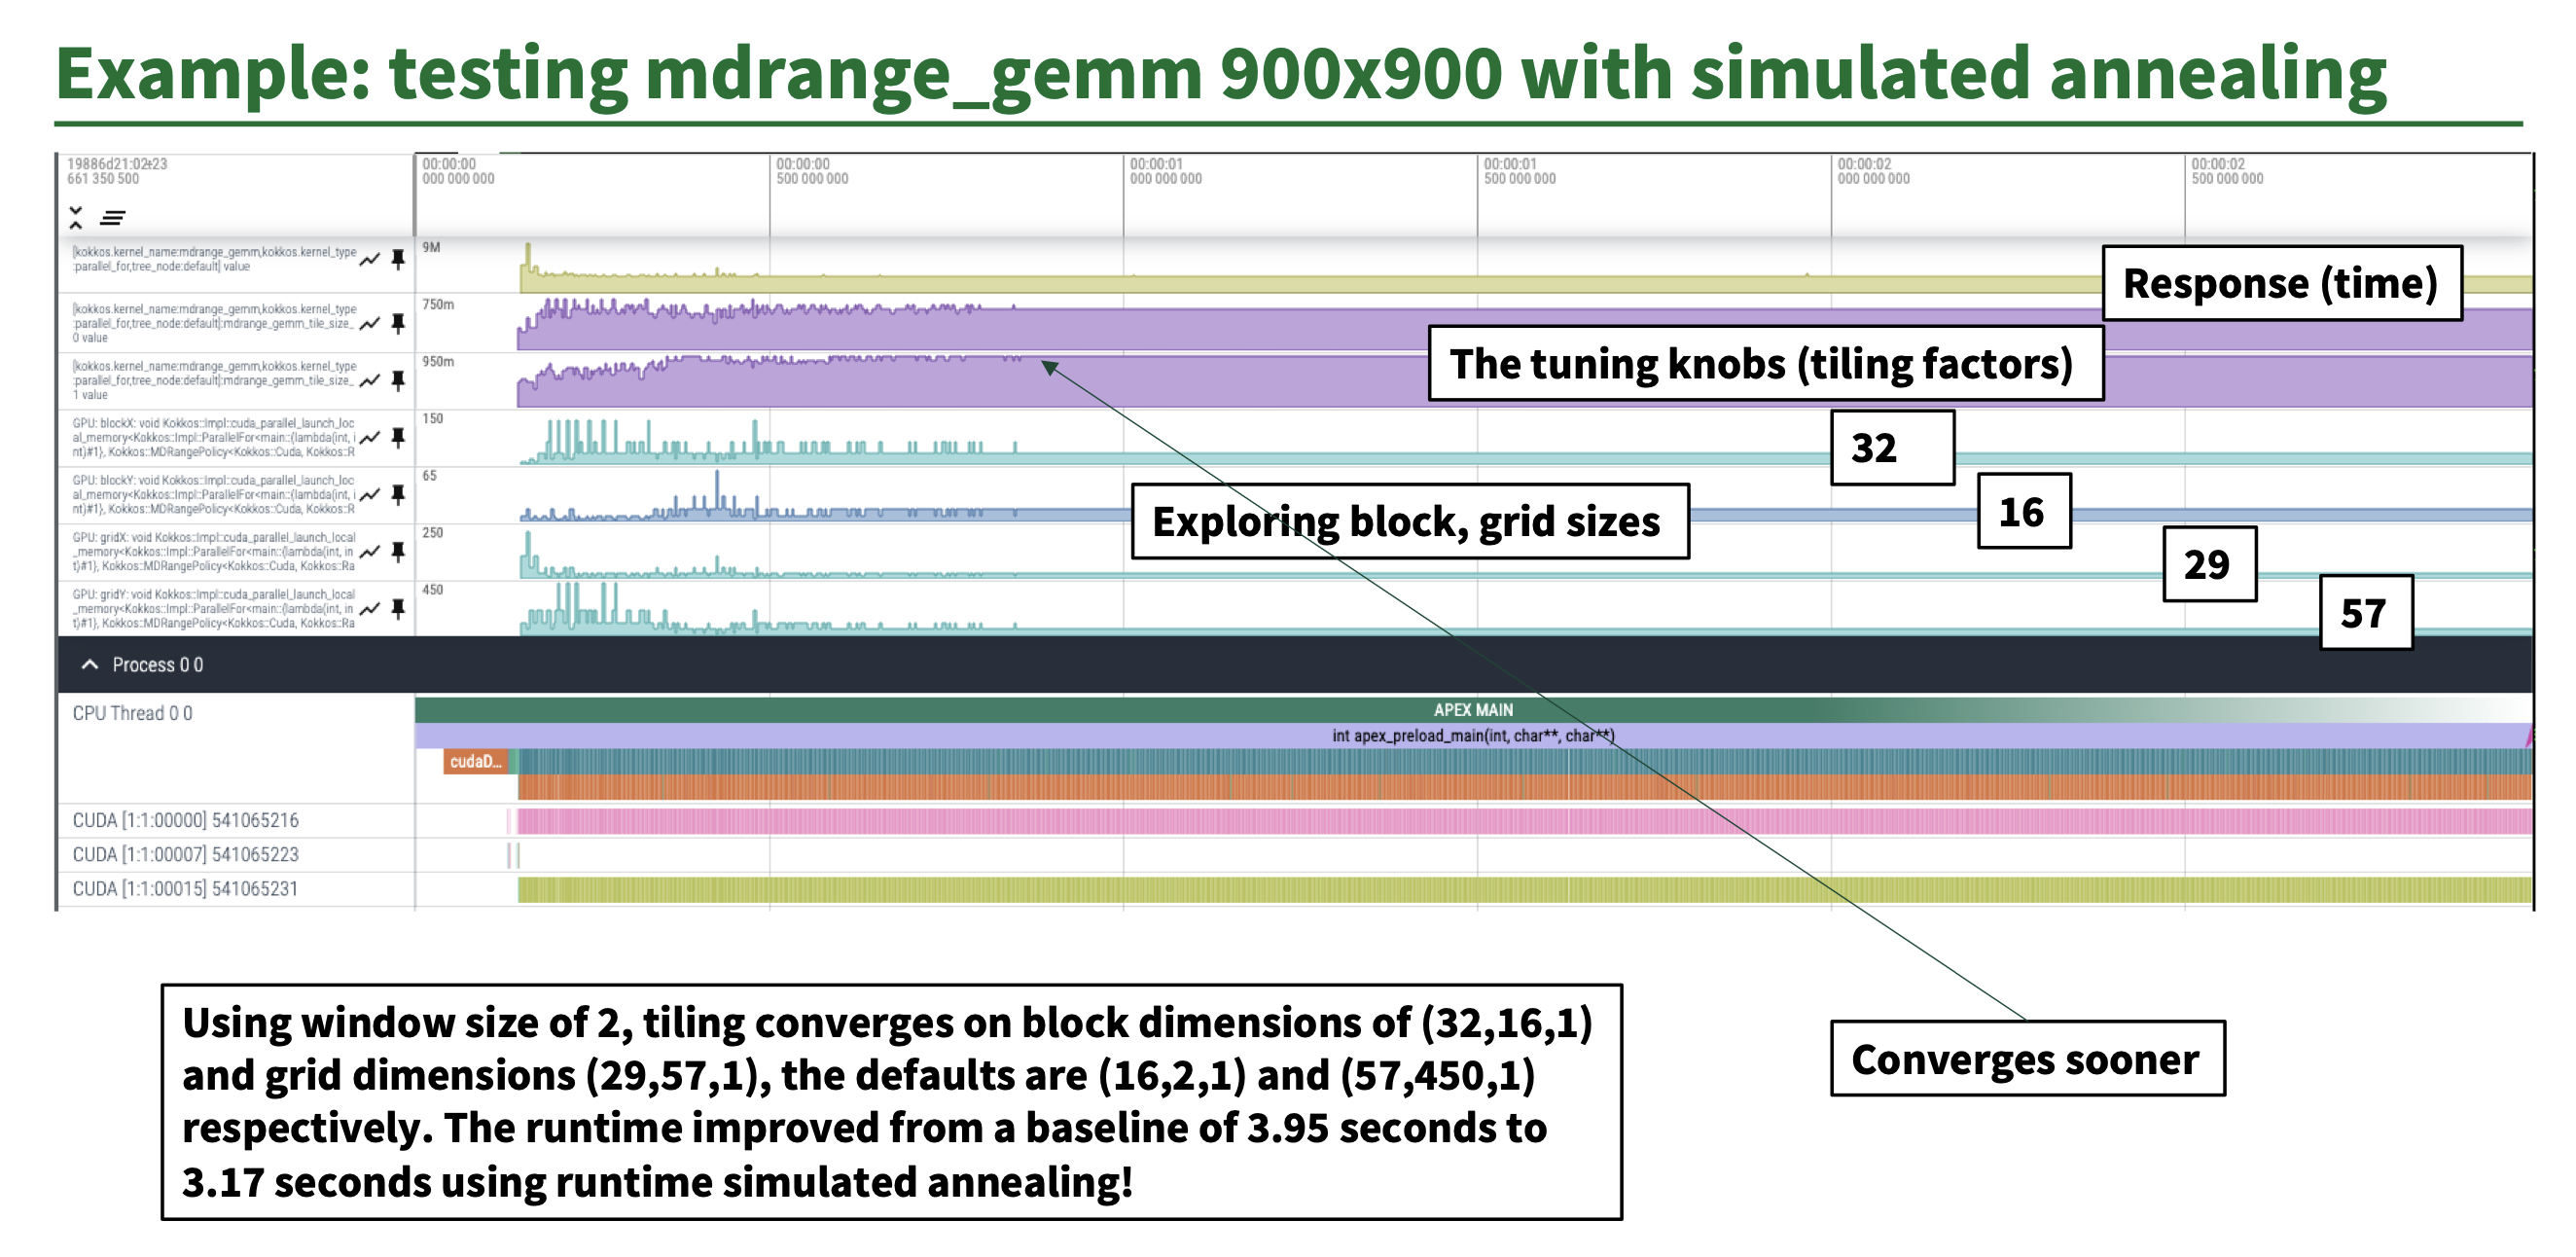
\includegraphics[width=\textwidth]{../figures/apextuningplot.png}
\end{figure}

\end{frame} 

\begin{frame}[fragile]{APEX In-depth}

\begin{center}
In-depth tutorial: \\
	\small \url{http://www.nic.uoregon.edu/~khuck/kokkos/2024-Kokkos-Tuning-Tutorial/2024-Kokkos-Tools-Tutorial-APEX.pdf}
\end{center}

\begin{center}
	Repo: \url{https://github.com/UA-OACISS/apex} \\	
	Email: \url{khuck@cs.uoregon.edu}
\end{center}

\end{frame}

\begin{frame}[fragile]{Apollo: a Prototype Tuning Tool}
  \textbf{Apollo: A model driven auto tuning tool}

\begin{itemize}
  \item Feature-rich tuning tool targeting this interface.
  \item Builds decision tree based models to find best-performing parameter values.
  \item Can retrain models if observed and expected performance deviate.
  \item Can save models for subsequent runs.
\end{itemize}

\pause
How to use Apollo:
	\begin{code}[mathescape=false]
export KOKKOS_TOOLS_LIBS=${APOLLO_PATH}/libapollo-tuner.so
./Executable.exe ARGS
\end{code}
\end{frame}

%======================================================================

\begin{frame}[fragile]{Some Results from the KokkosKernels Test Suite}
  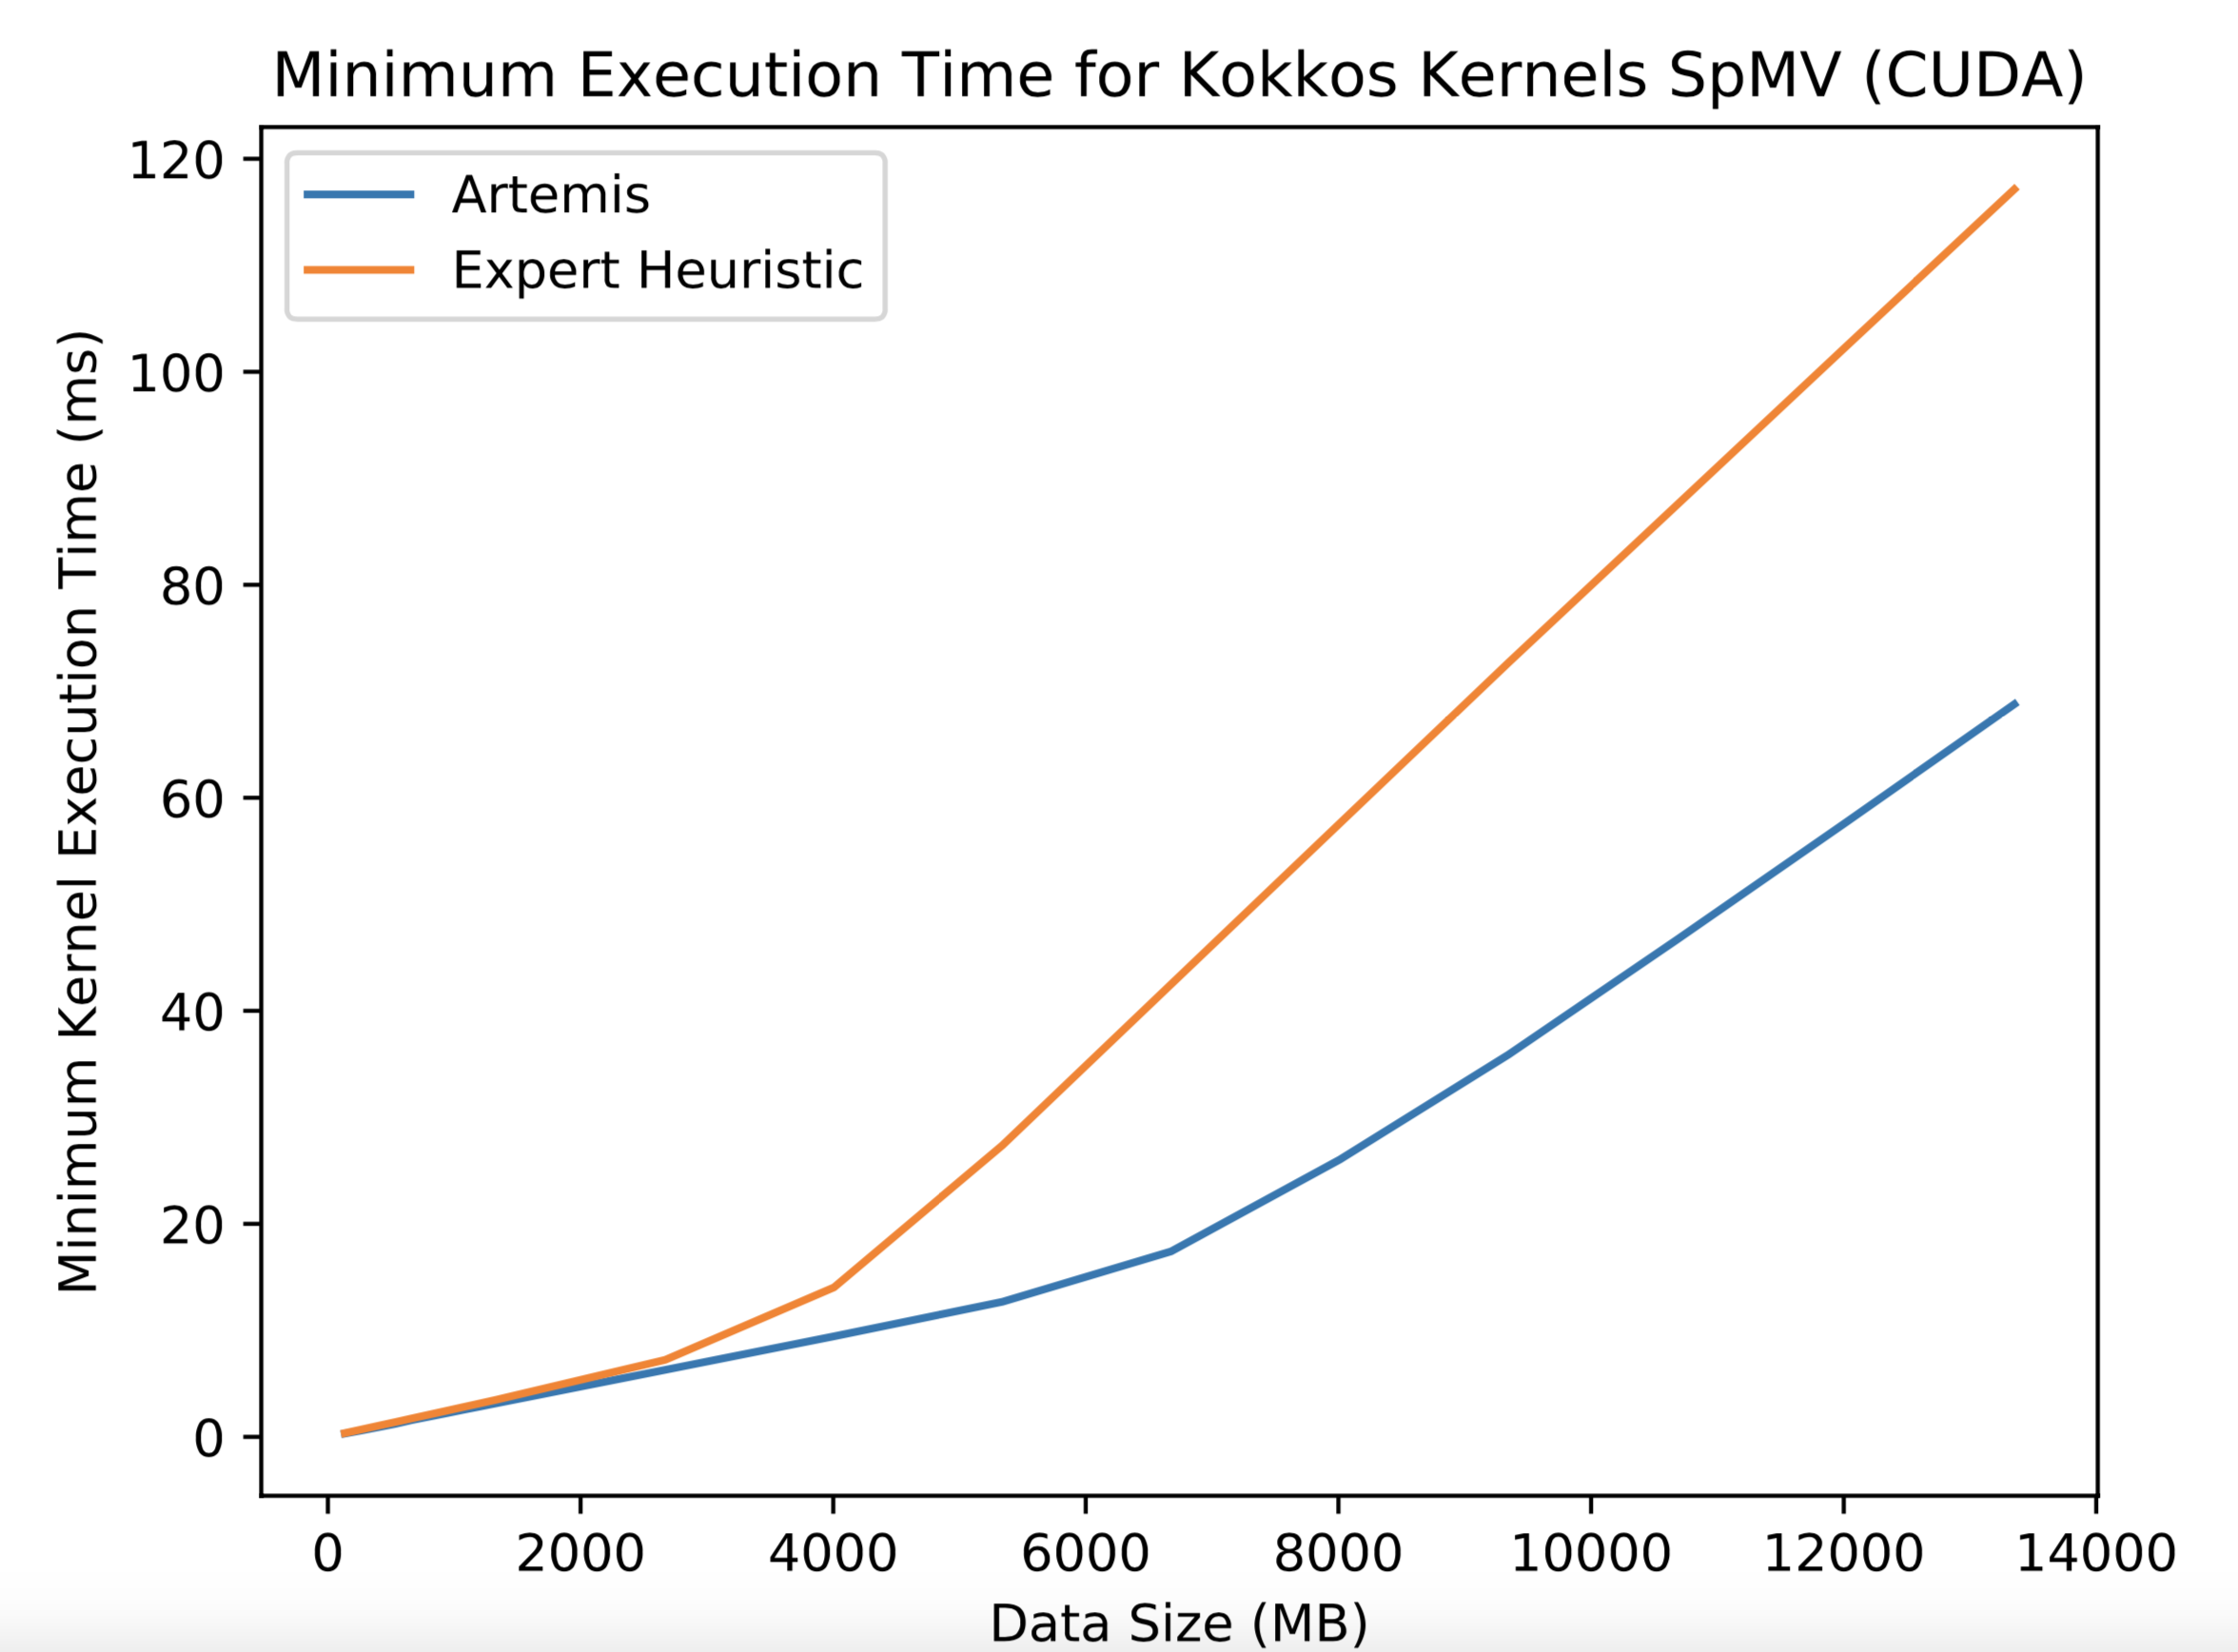
\includegraphics[width=0.9\textwidth]{../figures/apollo.png}
\end{frame}

\begin{frame}[fragile]{More Information on Apollo}

\begin{center} 
\textbf{Apollo Project Page:} \url{https://computing.llnl.gov/projects/apollo} \\
\end{center} 

\begin{center}
\textbf{Repo}: \url{https://github.com/LLNL/apollo} \\
\textbf{Contact}: \url{georgakoudis1@llnl.gov}
\end{center} 

\end{frame}

%==========================================================================

\begin{frame}[fragile]{Rules for Tuning}
  \begin{itemize}
    \item Load the output value array you pass to request\_output\_values
	    with sane defaults. If the tool doesn't overwrite them, your
	    program shouldn't crash. This protects you from a tool-free
	    situation
    \item No choice from your set/range of candidates should crash your
	    program. Options can be slow, but must all be functional
    \item Call set\_input\_values and request\_output\_values only once per context. 
  \end{itemize}
\end{frame}

\begin{frame}[fragile]{Future: Built-in Tuning}
For the future we plan on allowing automatic internal tuning of things like:
\begin{itemize}
  \item Team Size and Vector Length for \texttt{TeamPolicy}
  \item Tile Sizes for \texttt{MDRangePolicy}
  \item CUDA block size of \texttt{RangePolicy}
  \item Occupancy of kernels.
\end{itemize}
\begin{code}
parallel_for("A",TeamPolicy<>(N,AUTO,AUTO), ... );
parallel_for("B",MDRangePolicy<>({0,0},{N0,N1},{AUTO,AUTO}), ... );
\end{code}

\pause
But often more context is needed:
\begin{itemize}
  \item Kokkos on its own has limited information: Label, Iteration Range, and Kernel Type ID.
  \item SPMV: can't distinguish two matrices with same row count but vastly different row lengths.
  \item Stencil: can't distinguish runtime stencil depth.
\end{itemize}
\end{frame}


%==========================================================================

\begin{frame}[fragile]{Tuning Summary}
\textbf{Kokkos Tuning Hooks enable more performance portability}
\begin{itemize}
  \item Avoid figuring out the right heuristic for every platform.
  \item Will be more valuable when targeting Intel, NVIDIA and AMD GPUs as well as ARM, Intel, IBM and AMD CPUs!
\end{itemize}

\textbf{The app provides input variables to describe the context}
\begin{itemize}
  \item Input variables are descriptors of the problem scope.
  \item Categorical, Ranges, Sets are possible.
  \item Describe scaling for Ranges such as logarithmic or linear for categorizing problems.
\end{itemize}

\textbf{The app requests output variables}
\begin{itemize}
  \item Same type system as input variables.
  \item Enables the description of the search space for tools.
\end{itemize}

\end{frame}

